\documentclass[dvipdfmx,xcolor={svgnames},17pt]{beamer}

\usepackage{pxrubrica}
\usepackage{color}
\usepackage{tikz}
\usepackage{pgfplots}
\usepackage{amsmath}
\usepackage{amsfonts}
\usepackage{ifthen}
\usepackage{amsmath}

\usetikzlibrary{calc}
\pgfmathsetseed{20}

\setbeamertemplate{caption}[numbered]
\setbeamertemplate{footline}[frame number]

\renewcommand{\figurename}{図}
\renewcommand{\tablename}{表}

\pgfplotsset{
  integral axis/.style={
        axis lines=middle,
        enlarge y limits=upper,
        axis equal image, width=12cm,
        xlabel=$x$, ylabel=$y$,
        ytick=\empty,
        xticklabel style={font=\small, text height=1.5ex, anchor=north},
        samples=100
        },
        integral/.style={
            domain=2:10,
            samples=9
            },
            integral fill/.style={
            integral,
            draw=none, fill=#1,
            on layer=axis background
            },
            integral fill/.default=cyan!10,
            integral line/.style={
            integral,
            very thick,
            draw=#1
            },
            integral line/.default=black
}

\def\vector#1{\mbox{\boldmath $#1$}}

\renewcommand{\kanjifamilydefault}{\gtdefault} % 日本語書体をゴシック体に
\renewcommand{\familydefault}{\sfdefault} % 欧文書体をHelveticaに

\title{数値解析が\jruby{乱数}{み|だ}れる}
\author{13024156 藤原 渓亮}

\begin{document}

  \maketitle

  \begin{frame}{今日やること}
    \note{今日は乱数で定積分を解くモンテカルロ積分についてお話します.更に
    モンテカルロ積分に使う乱数の性能を上げた準乱数についてもお話します.
    }
    乱数で定積分を解く.\\
    準乱数で定積分を解く.
  \end{frame}

  \begin{frame}{数値積分とは}
    定積分を解析的にではなく数値的に解く
    \begin{block}{普通の積分}
      定積分 $\rightarrow$ 不定積分 $\rightarrow$ 解
    \end{block}
    \begin{block}{数値積分}
      定積分 $\rightarrow$ アルゴリズム $\rightarrow$ 近似解
    \end{block}
  \end{frame}

  \begin{frame}{数値積分の例}
    区分求積法
      台形公式
      シンプソンの公式
      シンプソンの3/8公式
  \end{frame}

  \begin{frame}{区分求積法}
    連続値 $\rightarrow$ 離散値 \\
    ex. 台形公式
    \begin{equation}
      \int^a_b f(x) dx \approx \sum_{k=0}^{n-1} \frac{\{f(x_{k+1}) + f(x_k)\}(x_{k+1}-x_k)}{2}
    \end{equation}
  \end{frame}

  \begin{frame}{区分求積法}
    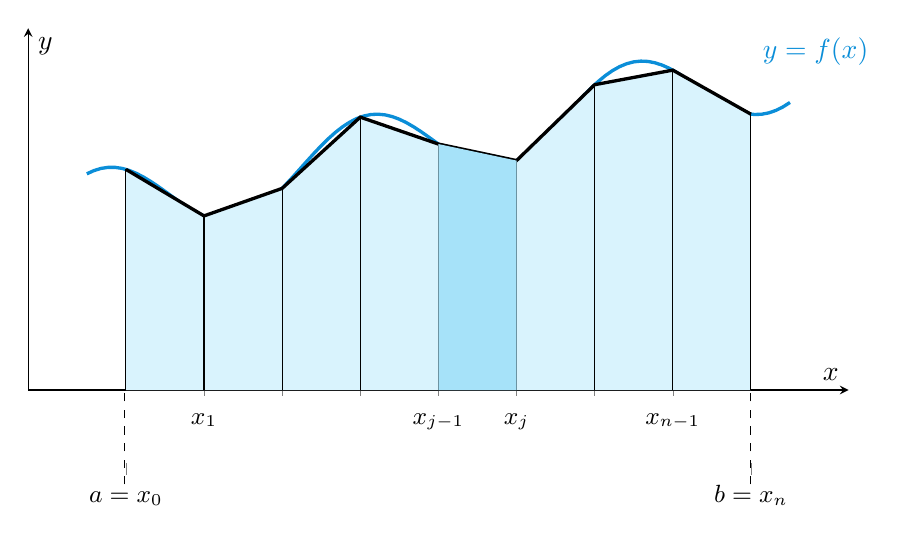
\begin{tikzpicture}[declare function={f=x/5-cos(deg(x*1.85))/2+2;}]
      \begin{axis}[
        integral axis,
        ymin=0,
        xmin=0.75, xmax=11.25,
        domain=1.5:10.5,
        xtick={3,...,9},
        extra x ticks={2,10},
        extra x tick labels={$a=x_0$, $b=x_n$},
        xticklabels={$x_1$,,,$x_{j-1}$,$x_j$,,$x_{n-1}$},
        extra x tick style={yshift=-1cm, anchor=south}
        ]

        % The function
        \addplot [very thick, cyan!75!blue] {f};

        % The filled area under the approximate integral
        \addplot [integral fill=cyan!15] {f} \closedcycle;

        % The approximate integral
        \addplot [integral line=black] {f};

        % The vertical lines between the segments
        \addplot [integral, ycomb] {f};

        % The highlighted segment
        \addplot [integral fill=cyan!35, domain=6:7, samples=2] {f} \closedcycle;
      \end{axis}
      \draw[dashed] (1.2275,-1.2) -- (1.2275,0);
      \draw[dashed] (9.175,-1.2) -- (9.175,0);
      \draw[cyan!75!blue] (10,4) node [above] {$y=f(x)$};
    \end{tikzpicture}
  \end{frame}

  \begin{frame}
    区分求積法なら計算機で計算できる. \\
    モンテカルロ積分の存在意義は? \\
    \pause
    $\rightarrow$ 重積分
    \pause
    \begin{equation}
      \idotsint f(x_1,x_2,\ldots x_L) dx_1dx_2\cdots dx_L
    \end{equation}
  \end{frame}

  \begin{frame}{区分求積法の計算量}
      L重積分をN個に分割するとき,計算量は \\
      $\rightarrow O(N^L)$
  \end{frame}

  \begin{frame}{乱数(列)とは}
    出力が一意的ではない数字のこと,法則性がない数列のこと
    \begin{itemize}
      \item 予測不可能性
      \item 一様性
      \item 非周期性
      \item 非再現性
    \end{itemize}
  \end{frame}

  \begin{frame}{予測不可能性}
    $x_0,x_1\ldots x_n$から$x_{n+1}$は予測できない.
  \end{frame}

    \begin{frame}{一様性}
      \begin{equation}
        P(x=X) = \frac{1}{\beta - \alpha} (\alpha \leq x \leq \beta)
      \end{equation}
      \begin{figure}[htbp]
        \centering
        \includegraphics[scale=0.3]{MTrand.png}
      \end{figure}
    \end{frame}

    \begin{frame}{非周期性}
      同じパターンの数列が現れない.
    \end{frame}

    \begin{frame}{非再現性}
      初期値が同じでも異なる数列が出現する.
    \end{frame}

    \begin{frame}{疑似乱数}
      厳密には決定的であるが乱数列のように見える数列
      \begin{itemize}
        \item 予測不可能性 $\rightarrow$ △
        \item 一様性 $\rightarrow$ △
        \item 非周期性 $\rightarrow$ x
        \item 非再現性 $\rightarrow$ x
      \end{itemize}
    \end{frame}

    \begin{frame}{予測不可能性 $\rightarrow$ △}
      ex) 線形合同法
      \begin{align}
        \vector{x} &= \{x_0,x_1,\ldots x_n, \ldots\} \\
        x_{n+1} &= (Ax_n + B) \bmod M (A,B,M \in \mathbb{Z})
      \end{align}
      $x_0,A,B,M$が分かれば予測可能
    \end{frame}

      \begin{frame}{一様性 $\rightarrow$ △}
        \begin{figure}[htbp]
          \includegraphics[scale=0.3]{lcm.jpg}
        \end{figure}
        粗悪なアルゴリズム $\rightarrow$ 高次元にて偏る.
      \end{frame}

      \begin{frame}{非周期性 $\rightarrow$ x}
        \begin{block}{線形合同法}
          $2^{32} - 1$
        \end{block}
        \begin{block}{$n$ビット線形帰還シフトレジスタ}
          $2^n - 1$
        \end{block}
        \begin{block}{メルセンヌ・ツイスタ}
          $2^{19937} - 1$
        \end{block}
        必ず,周期はある
      \end{frame}

      \begin{frame}{非再現性 $\rightarrow$ x}
        計算機の出力は決定的
      \end{frame}

      \begin{frame}{モンテカルロ積分}
        定積分をモンテカルロ法で解くこと
      \end{frame}

      \begin{frame}{モンテカルロ法とは}
        \begin{figure}
          \centering
          \includegraphics[scale=0.15]{monte.jpg}
          \caption{モナコ公国モンテカルロ地区}
          \label{fig:two}
        \end{figure}
      \end{frame}

      \begin{frame}{モンテカルロ法とは}
        乱数を用いて数値計算を行う方法
        乱択アルゴリズム
          モンテカルロ法 \visible<2,2>{一定の確率で誤る}
          ラスベガス法 \visible<2,2>{いつでも正答する}
      \end{frame}

      \begin{frame}{例題}
        \begin{minipage}{0.4\textwidth}
          \begin{equation}
            \int^1_0 \sqrt{1 - x^2}dx
          \end{equation}
          を解け
        \end{minipage}
        \begin{minipage}{0.5\textwidth}
          \centering
          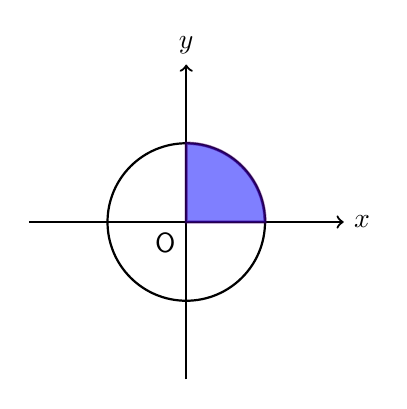
\begin{tikzpicture}[domain=0:8, samples=100, very thick] % 定義域、点の数、線幅
            \draw (0,0) node[below left]{O}; % 原点、0でも、above, below, left, rightで位置指定
            % 位置指定はanchor=north, south, east, westでも可能
            \draw[thick, ->] (-2,0)--(2,0) node[right] {$x$}; % x軸、[->]で矢印、他に[-stealth]等
            \draw[thick, ->] (0,-2)--(0,2) node[above] {$y$}; % y軸

            %\draw plot[domain=-1:1](\x, {sqrt(1-\x^2)}) node[above]{$f(x)=x^2-3x+2$}; % atでnodeの位置指定
            %\draw plot[domain=-1:1](\x, {-sqrt(1-\x^2)}) node[above]{$f(x)=x^2-3x+2$}; % atでnodeの位置指定
            \draw [thick] (0,0) circle (1);
            \filldraw [fill=blue, opacity=.5, draw=Indigo] (1,0)  arc (0:90:1) --(0,0)--cycle;
          \end{tikzpicture}
        \end{minipage}

      \end{frame}

      \begin{frame}
        \begin{align}
          &\int^1_0 \sqrt{1 - x^2}dx \\
          \intertext{$x = \cos\theta$と置く}
          &= \int^{1}_0 \sqrt{1 - \cos^2\theta} dx \\
          \intertext{$dx = -\sin\theta d\theta$より}
          &= \int^{\frac{\pi}{2}}_0 \sqrt{1 - \cos^2\theta}(-\sin\theta) d\theta
        \end{align}
      \end{frame}

      \begin{frame}
        \begin{align}
          &= -\int^{\frac{\pi}{2}}_0 \sin^2\theta d\theta \\
          \intertext{半角の公式より}
          &= -\frac{1}{2}\int^{\frac{\pi}{2}}_0 1 - 2\cos2\theta d\theta \\
          &= -\frac{1}{2}[\theta + \sin2\theta]^{\frac{\pi}{2}}_0 = \frac{\pi}{4}
        \end{align}
      \end{frame}

      \begin{frame}{モンテカルロ積分}
        \begin{tikzpicture}[declare function = {Circle(\x)= sqrt(5-\x)*sqrt(5+\x);}]
          \draw [] (0,0) rectangle (5,5);
          \draw [] (0,5)  arc (180:120:0.5);
          \draw [] (5,5)  arc (0:45:0.5);
          \draw (2.5,5.5) node {2};
          \draw [] (5,0)  arc (0:90:5) --(0,0)--cycle;
          \foreach \i in {1,...,2}
          {
            \foreach \j in {1,...,10}
            {
             \pgfmathsetmacro\myX{random(0,4) + random(0,1000)/1000}%
             \pgfmathsetmacro\myY{random(0,4) + random(0,1000)/1000}%
             \pgfmathsetmacro{\rndcolor}{ Circle(\myX)<\myY ? "red" : "blue" }
             \filldraw[fill=\rndcolor] (\myX, \myY) circle [radius=0.05];
            }
            \pause
          }
          \draw (9,5) node {青い点数 = $m$};
          \draw (9,4) node {赤い点数 = $n$};
          \draw (9,3) node {全体的な面積 = $4$};
          \draw (9,2) node {求めたい面積 = $x$};
          \draw (9,1) node {$m : n \approx x : 4$};
        \end{tikzpicture}
      \end{frame}

      \begin{frame}{演習}
        モンテカルロ積分のプログラムを \\
        完成させよ.
      \end{frame}

      \begin{frame}{休憩}
        続きは午後から
      \end{frame}

      \begin{frame}{準乱数}
        準乱数はランダム性を犠牲に一様性に特化した乱数の一種.
      \end{frame}

      \begin{frame}{van der corput列}
        基底$b$の逆基底関数$\phi_b$で定義される.
        \begin{align}
          \phi_b(n) = \sum_{ i\leq 0} d_ib^{-i-1} \\
          \{\phi_b(0), \phi_b(1), \phi_b(2), \ldots ,\phi_b(n)\}
        \end{align}
      \end{frame}

      \begin{frame}
        $d_i$は$n$を$b$進表記した時の$i$ビット目.
        \begin{align}
          10_{(10)} &= 1010_{(2)} \\
          d_0 &= 0 \\
          d_1 &= 1 \\
          d_2 &= 0 \\
          d_3 &= 1
        \end{align}
      \end{frame}

      \begin{frame}
        \begin{align}
          \phi_2(10) &= 1\times 2^{-3-1} + 0\times 2^{-2-1} + 1\times 2^{-1-1} + 0\times 2^{-0-1} \\
          &= \frac{1}{2^4} + \frac{1}{2^2} \\
          &= \frac{3}{8}
        \end{align}
      \end{frame}

      \begin{frame}{Halton列}
        van der corput列を高次元にしたもの
        \begin{align}
          X_n = \{\phi_{b1}(n), \phi_{b2}(n), \phi_{b3}(n), \ldots ,\phi_{b4}(n)\}
          \intertext{ただし,$b1,b2,\ldots ,bn$は全て素数}
        \end{align}
        今,求める積分は$x,y$の二次元なので二次元のHalton列($\vector{b} = \{2,3\}$)
      \end{frame}

      \begin{frame}{演習2}
        van der corput列を実装せよ.\\
        ヒント
        \begin{equation}
          vdc(b,n,i) = \frac{(n\bmod b)}{b^{i+1}} + vdc(b, \frac{n}{b}, i+1))
        \end{equation}
      \end{frame}

      \begin{frame}{演習3}
        準モンテカルロ法を完成させよ.\\
      \end{frame}



\end{document}
